\documentclass[twocolumn,english]{article}
\usepackage[latin9]{inputenc}
\usepackage[landscape]{geometry}
\geometry{verbose,tmargin=0.5in,bmargin=0.75in,lmargin=0.5in,rmargin=0.5in}
\setlength{\parskip}{0bp}
\setlength{\parindent}{0pt}
\usepackage{array}
\usepackage{float}
\usepackage{booktabs}
\usepackage{multirow}
\usepackage{amsbsy}
\usepackage{graphicx}

\makeatletter

\providecommand{\tabularnewline}{\\}

\setlength{\columnsep}{0.25in}
\usepackage{xcolor}
\usepackage{textcomp}
\usepackage{listings}
\lstset{
  language=haskell,
  tabsize=2,
  basicstyle=\small\ttfamily,
}

\makeatother

\usepackage{babel}
\usepackage{listings}
\renewcommand{\lstlistingname}{Listing}

\begin{document}

\title{Reference Sheet for C113 Architecture}


\date{Spring 2017}

\maketitle

\part{Hardware and Representation}


\section{Integers and Characters}


\subsection{Unsigned Integer Representation}

For a number $d_{n}d_{n-1}\dots d_{0}$ in base $b$ we have $\sum_{k=0}^{n}d_{k}\times b^{k}$.

Hence $n$ bits can represent $2^{n}-1$ unsigned integers.


\paragraph{Converting from Decimal to Binary}
\begin{enumerate}
\item Divide the number by 2, writing down the quotient and remainder.
\item Repeat this process on the quotient until 0 is reached.
\item The binary number is obtained by reading the remainders from bottom
to top.
\end{enumerate}

\paragraph{Converting between Binary and Octal}

Simply convert from the least significant bit:

000 (0), 001 (1), 010 (2), 011 (3), 100 (4), 101 (5), 110 (6), 111
(7).


\paragraph{Converting between Binary and Hexadecimal}

Simply convert from the least significant bit:

0000 (0), 0001 (1), 0010 (2), 0011 (3), 0100 (4), 0101 (5), 0110 (6),
0111 (7), 1000 (8), 1001 (9), 1010 (A), 1011 (B), 1100 (C), 1101 (D),
1110 (E), 1111 (F).


\paragraph{Radix Arithmetic}

Exactly as for decimal but use the base (2 for binary) as point of
reference instead of 10.


\paragraph{Bit Groups}

Bit (1), Byte (8), Word (usually 16, 32 or 64).


\subsection{Signed Integer Representation}


\paragraph{Sign and Magnitude}

0 for positive, 1 for negative, followed by value. Has several disadvantages:
\begin{enumerate}
\item Two bit patterns for 0, which wastes a value and requires hardware
to treat both values as 0.
\item Explicitly need to implement substractors and adders, so more costly
to implement.
\end{enumerate}

\paragraph{One's Complement}

Invert each bit for negative. Still two bit patterns for 0, which
means result after operation not always correct.


\paragraph{Two's complement}

Complement each bit and add 1 to result.
\begin{enumerate}
\item $-X\mbox{ defined as }2^{n}-X$
\item $X+\bar{X}=1\dots111_{2}=-1\iff-X=\bar{X}+1$
\item $n$ bits can represent any integer in the range from $-2^{n-1}$
to $2^{n-1}-1$.
\end{enumerate}

\paragraph{Excess $\boldsymbol{n}$}

Represent $X$ as $X+n$


\paragraph{Binary Coded Decimal}

Each nibble (4 bits) encodes value from 0 - 9. Sign nibble at end
(1100 for + or 1101 for -).


\paragraph{Arithmetic}
\begin{enumerate}
\item \emph{Addition}: Add and discard carry bit.
\item \emph{Subtraction}: Negate subtrahend, add as before.
\item \emph{Overflow}: For two numbers which are both positive or both negative,
overflow occurs iff the result has opposite sign.
\end{enumerate}

\subsection{Character Representation}

ASCII (7 or 8 bits) or Unicode.


\section{Memory}


\subsection{Register Memory}
\begin{enumerate}
\item Few small memories located in CPU, but very fast.
\item Includes general purpose registers and special purpose registers (internal
to CPU or accessed with special instructions).
\item Referenced directly by specific instructions or encoding register
number within instructions.
\item Contents lost when CPU turned off.
\end{enumerate}

\subsection{Disk Memory}
\begin{enumerate}
\item Contents not lost when turned off, but much slower than other memories.
\item Locations identified by special addressing schemes.
\end{enumerate}

\subsection{Main Memory}
\begin{enumerate}
\item Slower than register memory but still fast. \emph{Access time} is
time to read or write, is constant for all locations.
\item Used to hold both program code (instructions) and data (numbers, strings,
...)
\item Locations identified by \emph{addressing scheme}, numbering bytes
from 0 onwards.
\item Contents lost when power turned off.
\end{enumerate}

\subsubsection{Types of Main Memory}
\begin{enumerate}
\item \emph{Static Random Access Memory}: Fast but expensive, used for cache
memory.
\item \emph{Dynamic RAM}: Cheaper, used for main memory, needs to be refreshed
every few milliseconds (due to transistors losing charge).
\item \emph{Synchronous DRAM}: Type of DRAM synchronised with clock of CPU's
system bus.
\item \emph{Double-Data Rate SDRAM}: Allows data to be transferred on both
rising edge and falling edge.
\item \emph{Read Only Memory}: Semiconductor, can only be written to once.
\item \emph{Programmable ROM}: Allows end users to write (once).
\item \emph{Erasable PROM}: Can erase using strong UV light, contents and
rewrite, usually stores boot program (firmware): BIOS (Basic I/O System)
/ EFI (Extensible Firmware Interface).
\item \emph{Electrically EPROM}: Erased electrically.
\item \emph{FLASH}: Cheaper EEPROM, but updates can only be performed on
blocks, not individual bytes.
\end{enumerate}

\subsubsection{Organisation of Main Memory}
\begin{enumerate}
\item Consider as a matrix of bits. 
\item Each row represents a memory row (with a natural number giving its
\emph{address}, used to select row). 
\item Often row is word-size of architecture, can be half or multiple. 
\item We assume data can only be read or written to single row
\end{enumerate}

\subsubsection{Byte Addressing}

Many architectures make main memory byte-addressable rather than word
addressable. Two approaches to ordering:
\begin{enumerate}
\item \emph{Big-Endian}: Most significant byte has lowest address.
\item \emph{Little-Endian}: Least significant byte has the lowest address.
\end{enumerate}
\noindent 
\begin{table}[H]
\noindent \centering{}%
\begin{tabular}{cccccccccc}
 & \multicolumn{4}{c}{Big Endian} &  & \multicolumn{4}{c}{Little Endian}\tabularnewline
 & \multicolumn{4}{c}{MSB $\rightarrow$ LSB} &  & \multicolumn{4}{c}{MSB $\rightarrow$ LSB}\tabularnewline
 & 24 & 25 & 26 & 27 &  & 27 & 26 & 25 & 24\tabularnewline
\cline{2-5} \cline{7-10} 
\multicolumn{1}{c|}{Word 24} & 12 & 2E & 5F & \multicolumn{1}{c|}{01} & \multicolumn{1}{c|}{Word 24} & 12 & 2E & 5F & \multicolumn{1}{c|}{01}\tabularnewline
\cline{2-5} \cline{7-10} 
\end{tabular}
\end{table}


\emph{Important}: ASCII bytes are treated independently.

\noindent 
\begin{table}[H]
\noindent \centering{}%
\begin{tabular}{cccccccccc}
 & \multicolumn{4}{c}{Big Endian} &  & \multicolumn{4}{c}{Little Endian}\tabularnewline
 & \multicolumn{4}{c}{MSB $\rightarrow$ LSB} &  & \multicolumn{4}{c}{MSB $\rightarrow$ LSB}\tabularnewline
 & +0 & +1 & +2 & +3 &  & +3 & +2 & +1 & +0\tabularnewline
\cline{2-5} \cline{7-10} 
\multicolumn{1}{c|}{Word 24} & S & T & R & \multicolumn{1}{c|}{I} & \multicolumn{1}{c|}{Word 24} & I & R & T & \multicolumn{1}{c|}{S}\tabularnewline
\multicolumn{1}{c|}{Word 28} & N & G & ? & \multicolumn{1}{c|}{?} & \multicolumn{1}{c|}{Word 28} & ? & ? & G & \multicolumn{1}{c|}{N}\tabularnewline
\cline{2-5} \cline{7-10} 
\end{tabular}
\end{table}



\subsubsection{Word Allignment}
\begin{enumerate}
\item Some architectures allow any word-sized bit group regardless of byte
address.
\item \emph{Aligned access}: acess begins on memory word boundary.
\item \emph{Unaligned access}: does not. Slow because requires reading of
required bits from adjacent words and concatenating together.
\end{enumerate}

\subsubsection{Modules and Chips}
\begin{enumerate}
\item RAM comes physcially in \emph{modules}, each comprised of several
\emph{chips}.
\item \emph{DIMMs} (dual inline memory modules) support 64-bit transfers,
\emph{SIMMs} support 32-bit.
\item A chip with length $2^{k}$ requires $k$ address bits.
\item Number of chips = size of memory $/$ size of chip.
\item Chips per module $=$ width of memory word $/$ width of chip.
\item Number of modules = number of chips $/$ chips per module.
\end{enumerate}
E.g. 1M$\times$16 bit main memory made of 256K$\times$4 bit chips
has 16 chips, 4 chips per module, 4 modules.


\subsubsection{Interleaved Memory}

Some address bits select module, and remaining bits select row.
\begin{enumerate}
\item \emph{Low-order interleaved memory}: Module selection bits are least
significant bits in memory address.
\item \emph{High-order interleaved}: Module selection bits are most significant
bits.
\item If more than one module can be read/written at a time:

\begin{enumerate}
\item Low-order: Read same row in each module. E.g. single multi-word access
of sequential data.
\item High-order: Different modules independently accessed by different units.
E.g. CPU can access rows in one module, hard disk / another CPU access
row in another module concurrently.
\end{enumerate}
\end{enumerate}

\section{The CPU}
\begin{enumerate}
\item Consider the task $A=B+C$. We compile this into a sequence of \emph{assembly
instructions}: LOAD R2 B. ADD R2, C. STORE R2, A. (where A, B, C designate
memory locations)
\item Consider also an architecture with 16-bit words, 4 general purpose
registers (R0, R1, R2, R3), 16 different instructions in its \emph{instruction
set}, represents integers using two's complement.
\item Consider finally an \emph{instruction format} with: 4 bits for OPCODE
(identifies CPU operation), 2 bits for REG (defines a general purpose
register), 10 bits for ADDRESS (defines address of word in RAM).
\end{enumerate}

\paragraph{Von Neumann Machine Model}
\begin{enumerate}
\item 3 subsystems: CPU, main memory, I/O system.
\item Main memory holds program as well as data.
\item Instructions are executed sequentially.
\item Single path exists between control unit and main memory, leads to
von Neumann bottleneck.
\end{enumerate}

\subsection{CPU Organisation}

\begin{figure}[H]
\noindent \centering{}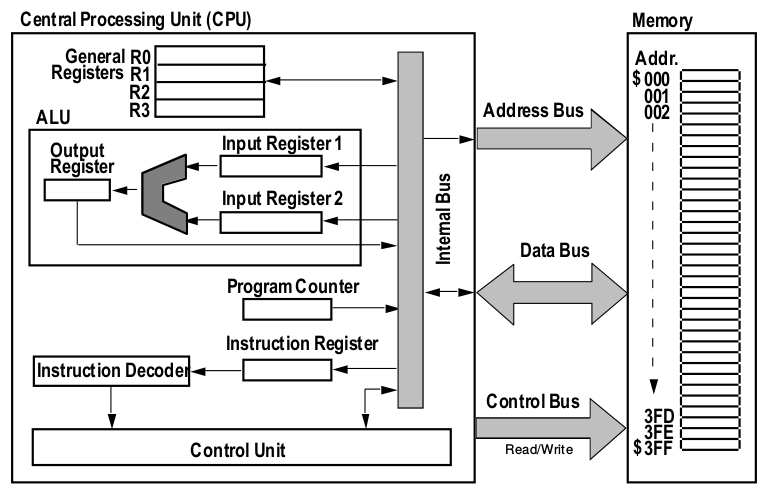
\includegraphics[scale=0.35]{img/cpu}
\end{figure}

\begin{enumerate}
\item \emph{PC}: Holds address of next instruction to be fetched from memory.
\item \emph{IR}: Holds each instrcution after being fetched.
\item \emph{Instruction Decoder}: Decodes (splits) contents of IR for control
unit to interpret.
\item \emph{Control unit}: Co-ordinates activity in CPU. Connected to all
parts of CPU, includes timing circuit.
\item \emph{ALU}: Carries out arithmetic and logical operations.

\begin{enumerate}
\item \emph{ALU Input Registers 1 \& 2}: Holds operands for ALU.
\item \emph{ALU Output register}: Holds result of ALU operation. Result
is then copied to final destination (e.g. CPU register, main memory,
I/O device).
\end{enumerate}
\item \emph{General-Purpose Registers}: For use by programmer.
\item \emph{Buses}: Pass information within CPU and between CPU and main
memory. Generally transfer $>$1 bit at a time.

\begin{enumerate}
\item \emph{Address Bus}: sends address from CPU to main memory, indicates
address in memory to read/write to.
\item \emph{Data Bus}: bidirectional, sends a word from CPU to main memory
or vice versa.
\item \emph{Control bus}: indicates whether CPU is reading or writing, i.e.
direction of data bus.
\end{enumerate}
\end{enumerate}

\subsection{The Fetch-Execute Cycle}
\begin{enumerate}
\item \emph{Fetch Instruction and Increment Program Counter. Eg.:}

\begin{enumerate}
\item Address goes from PC to address bus.
\item Control bus set to 0.
\item Address goes from address bus to memory.
\item 0 goes from control bus to memory (so READ).
\item PC incremented.
\item Instruction goes from memory{[}address{]} to data bus.
\item Instruction goes from data bus to IR.
\end{enumerate}
\item \emph{Decode Instruction. E.g.:}

\begin{enumerate}
\item Instruction goes from IR to instruction decoder.
\item OPCODE, REG and ADDRESS go from decoder to control unit.
\end{enumerate}
\item \emph{Execute Instruction (Fetch Operands, Perform Operation, Store
Results). E.g. LOAD:}

\begin{enumerate}
\item ADDRESS goes from control unit to address bus.
\item Control bus set to 0.
\item ADDRESS goes from address bus to memory.
\item 0 goes from control bus to memory (so READ).
\item Value goes from Memory{[}ADDRESS{]} to data bus.
\item Value goes from data bus to REG.
\end{enumerate}
\item \emph{E.g. ADD:}

\begin{enumerate}
\item Value 1 goes from REG to ALU input reg 1.
\item ADDRESS goes from control unit to address bus.
\item Control bus set to 0.
\item ADDRESS goes from address bus to memory.
\item 0 goes from control bus to memory (so READ).
\item Value 2 goes from memory{[}ADDRESS{]} to data bus.
\item Value 2 goes from data bus to ALU reg 2.
\item Operation goes from control unit to ALU (so ADD).
\item Final value goes from ALU output reg to REG.
\end{enumerate}
\item \emph{E.g. WRITE:}

\begin{enumerate}
\item Value goes from REG to data bus.
\item ADDRESS goes from control unit to address bus.
\item Control bus set to 1.
\item Value goes from data bus to memory.
\item ADDRESS goes from address bus to memory.
\item 1 goes from control bus to memory (so WRITE).
\end{enumerate}
\item \emph{Repeat Forever}
\end{enumerate}

\subsection{Assembly Code}

Consider a basic instruction set:

\begin{table}[H]
\noindent \centering{}%
\begin{tabular}{clrl}
\toprule 
\emph{OP Code} & \multicolumn{2}{c}{\emph{Assembler Format}} & \emph{Action}\tabularnewline
\midrule
0000 & STOP &  & Stop execution\tabularnewline
0001 & LOAD & Rn, {[}addr{]} & Rn = Memory{[}addr{]}\tabularnewline
0010 & STORE & Rn, {[}addr{]} & Memory{[}addr{]} = Rn\tabularnewline
0011 & ADD & Rn, {[}addr{]} & Rn = Rn + Memory{[}addr{]}\tabularnewline
0100 & SUB & Rn, {[}addr{]} & Rn = Rn - Memory{[}addr{]}\tabularnewline
1010 & GOTO & addr & PC = addr\tabularnewline
0110 & IFZER & Rn, addr & IF Rn = 0 THEN PC = addr\tabularnewline
0111 & IFNEG & Rn, addr & IF Rn \textless{} 0 THEN PC = addr\tabularnewline
1001 & LOAD & Rn, {[}Rm{]} & Rn = Memory{[}Rm{]}\tabularnewline
1010 & STORE & Rn, {[}Rm{]} & Memory{[}Rm{]} = Rn\tabularnewline
1011 & ADD & Rn, {[}Rm{]} & Rn = Rn + Memory{[}Rm{]}\tabularnewline
1100 & SUB & Rn, {[}Rm{]} & Rn = Rn - Memory{[}Rm{]}\tabularnewline
\bottomrule
\end{tabular}
\end{table}


\begin{table}[H]
\textbf{Example 1: Multiplication\smallskip{}
}

\noindent \begin{minipage}[b]{0.15\textwidth}
\begin{lstlisting}[basicstyle={\scriptsize},breaklines=true,keywords={loop, exit, when, end}]
; Given A, B, C
; Pre: C >= 0
; Post A = B * C

sum = 0
n = C
loop
    exit when n <= 0
    sum = sum + B
    n = n - 1
end loop
A = sum
\end{lstlisting}


\noindent \end{minipage}
\begin{minipage}[b]{0.35\textwidth}%
\begin{tabular}{clrl}
\toprule 
\emph{\footnotesize{}Address} & \multicolumn{2}{c}{\emph{\footnotesize{}Assembler Instruction}} & \emph{\footnotesize{}Comment}\tabularnewline
\midrule
{\footnotesize{}80H} & {\footnotesize{}LOAD} & {\footnotesize{}R1, {[}200H{]}} & {\footnotesize{}; sum = 0}\tabularnewline
{\footnotesize{}81H} & {\footnotesize{}LOAD} & {\footnotesize{}R2, {[}102H{]}} & {\footnotesize{}; n = C}\tabularnewline
{\footnotesize{}82H} & {\footnotesize{}IFZER } & {\footnotesize{}R2, 87H} & {\footnotesize{}; }\textbf{\footnotesize{}exit when}{\footnotesize{}
n = 0}\tabularnewline
{\footnotesize{}83H} & {\footnotesize{}IFNEG} & {\footnotesize{}R2, 87H} & {\footnotesize{}; }\textbf{\footnotesize{}exit when}{\footnotesize{}
n \textless{} 0}\tabularnewline
{\footnotesize{}84H} & {\footnotesize{}ADD} & {\footnotesize{}R1, {[}101H{]}} & {\footnotesize{}; sum = sum + B}\tabularnewline
{\footnotesize{}85H} & {\footnotesize{}SUB} & {\footnotesize{}R2, {[}201H{]}} & {\footnotesize{}; n = n - 1}\tabularnewline
{\footnotesize{}86H} & {\footnotesize{}GOTO} & {\footnotesize{}82H} & {\footnotesize{}; }\textbf{\footnotesize{}end loop}\tabularnewline
{\footnotesize{}87H} & {\footnotesize{}STORE} & {\footnotesize{}R1, {[}100H{]}} & {\footnotesize{}; A = sum}\tabularnewline
{\footnotesize{}88H} & {\footnotesize{}STOP} &  & {\footnotesize{}; end of program}\tabularnewline
\midrule
{\footnotesize{}100H} & {\footnotesize{}A} &  & {\footnotesize{}; Holds A}\tabularnewline
{\footnotesize{}101H} & {\footnotesize{}B} &  & {\footnotesize{}; Holds B}\tabularnewline
{\footnotesize{}102H} & {\footnotesize{}C} &  & {\footnotesize{}; Holds C}\tabularnewline
\midrule
{\footnotesize{}200H} & {\footnotesize{}0} &  & {\footnotesize{}; Holds 0}\tabularnewline
{\footnotesize{}201H} & {\footnotesize{}1} &  & {\footnotesize{}; Holds 1}\tabularnewline
\bottomrule
\end{tabular}

\noindent \centering{}\end{minipage}
\end{table}
\begin{table}[H]
\noindent \textbf{Example 2: Vector Sum\smallskip{}
}

\noindent \begin{minipage}[b]{0.18\textwidth}
\begin{lstlisting}[basicstyle={\scriptsize},breaklines=true,keywords={loop, exit, when, end}]
sum = 0
n = 100
addr = 200H
loop
    exit when n <= 0
    sum = sum + RAM[addr]
    addr = addr + 1
    n = n - 1
end loop
; Result in Register R0
\end{lstlisting}


\noindent \end{minipage}
\begin{minipage}[b]{0.32\textwidth}%
\begin{tabular}{clrl}
\toprule 
\emph{\footnotesize{}Address} & \multicolumn{2}{c}{\emph{\footnotesize{}Assembler Instruction}} & \emph{\footnotesize{}Comment}\tabularnewline
\midrule 
{\footnotesize{}0} & {\footnotesize{}0} &  & {\footnotesize{}; Holds 0}\tabularnewline
{\footnotesize{}1} & {\footnotesize{}1} &  & {\footnotesize{}; Holds 1}\tabularnewline
{\footnotesize{}2} & {\footnotesize{}100} &  & {\footnotesize{}; Holds 100}\tabularnewline
{\footnotesize{}3} & {\footnotesize{}200H} &  & {\footnotesize{}; Holds 200H}\tabularnewline
\midrule
{\footnotesize{}0FH} & {\footnotesize{}LOAD} & {\footnotesize{}R0, {[}0{]}} & {\footnotesize{}; sum = 0}\tabularnewline
{\footnotesize{}10H} & {\footnotesize{}LOAD} & {\footnotesize{}R1, {[}2{]}} & {\footnotesize{}; n = 100}\tabularnewline
{\footnotesize{}11H} & {\footnotesize{}LOAD} & {\footnotesize{}R2, {[}3{]}} & {\footnotesize{}; addr = 200H}\tabularnewline
{\footnotesize{}12H} & {\footnotesize{}IFZER} & {\footnotesize{}R1, 18H} & {\footnotesize{}; }\textbf{\footnotesize{}exit when}{\footnotesize{}
n = 0}\tabularnewline
{\footnotesize{}13H} & {\footnotesize{}IFNEG} & {\footnotesize{}R1, 18H} & {\footnotesize{}; }\textbf{\footnotesize{}exit when}{\footnotesize{}
n \textless{} 0}\tabularnewline
{\footnotesize{}14H} & {\footnotesize{}ADD} & {\footnotesize{}R0, {[}R2{]}} & {\footnotesize{}; sum = sum + ...}\tabularnewline
{\footnotesize{}15H} & {\footnotesize{}ADD} & {\footnotesize{}R2, {[}1{]}} & {\footnotesize{}; addr = addr + 1}\tabularnewline
{\footnotesize{}16H} & {\footnotesize{}SUB} & {\footnotesize{}R1, {[}1{]}} & {\footnotesize{}; n = n - 1}\tabularnewline
{\footnotesize{}17H} & {\footnotesize{}GOTO} & {\footnotesize{}12H} & {\footnotesize{}; }\textbf{\footnotesize{}end loop}\tabularnewline
{\footnotesize{}18H} & {\footnotesize{}STOP} &  & {\footnotesize{}; end of program}\tabularnewline
\bottomrule
\end{tabular}

\noindent \centering{}\end{minipage}
\end{table}



\subsection{The Control Unit}


\subsubsection{CPU Structure}

\begin{figure}[H]
\noindent \centering{}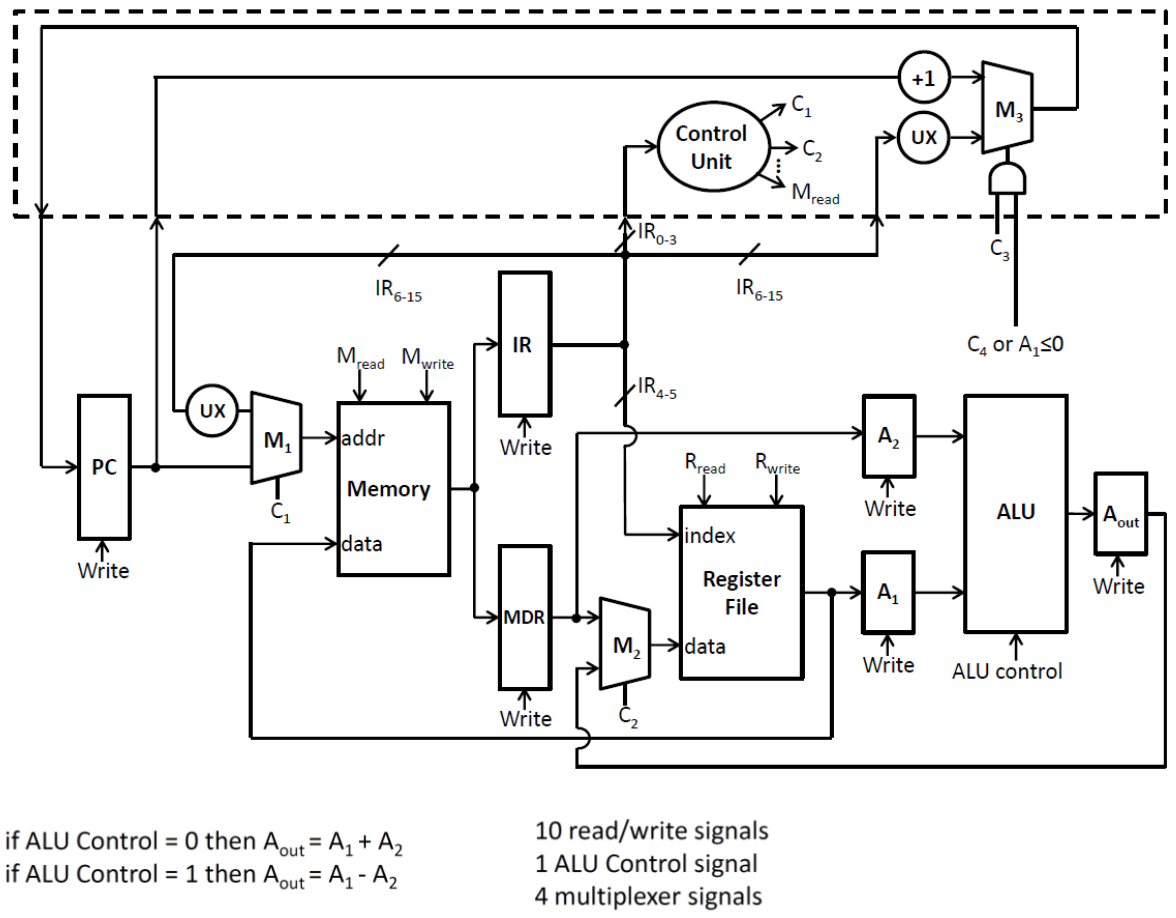
\includegraphics[scale=0.2]{img/cpu-hardware}
\end{figure}

\begin{enumerate}
\item Registers respond in next cycle.
\item Combinatorial components respond in same cycle.
\end{enumerate}

\subsubsection{Micro-Steps}

\begin{figure}[H]
\noindent \centering{}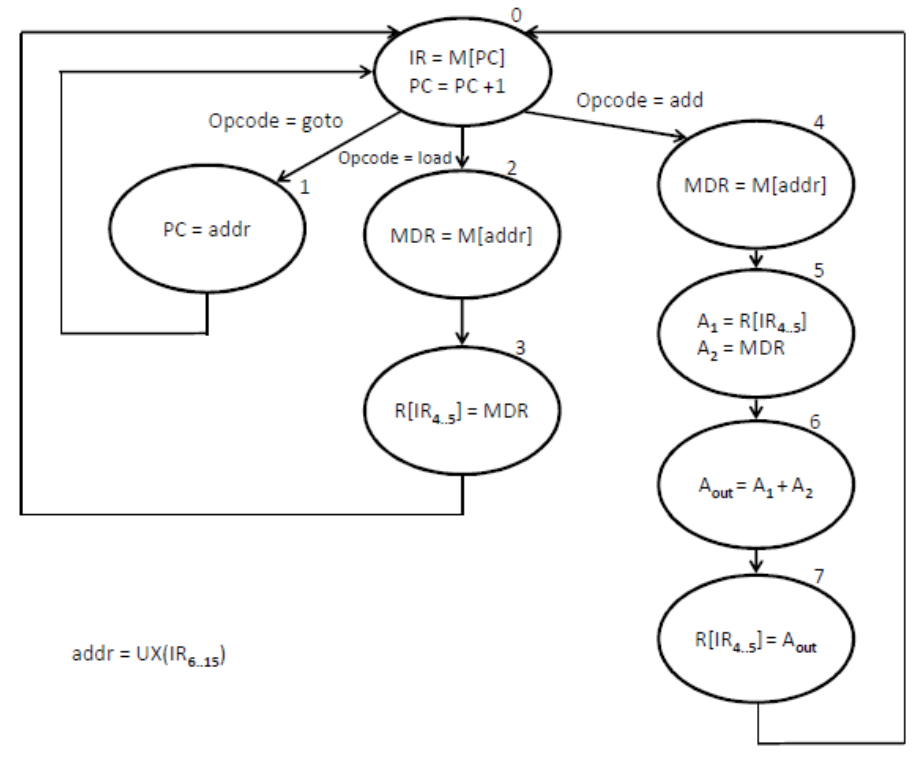
\includegraphics[scale=0.275]{img/microsteps}
\end{figure}

\begin{enumerate}
\item \emph{Required Inputs}: One of 16 opcodes (4 bits), one of 8 states
(3 bits).
\item \emph{Required Outputs}: 15 control signals (see circuit diagram),
next state (3 bits).
\end{enumerate}

\paragraph{ROM Implementation}

7 bits input, 18 bits output so size is $2^{7}\times18$.

\begin{figure}[H]
\noindent \centering{}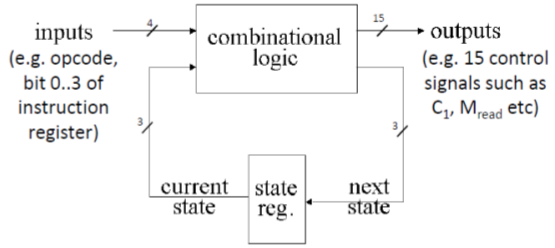
\includegraphics[scale=0.325]{img/rom-implementation}
\end{figure}



\paragraph{Microsequencer Implementation}
\begin{enumerate}
\item Micro-program counter used to keep track of current state.
\item Multiplexer chooses: 0 - next instruction, 1 - choose based on opcode,
2 - increment by one.
\item \emph{Instruction Decode ROM}: 4 inputs, 3 outputs so size $2^{4}\times3$.
\item \emph{Control Logic ROM}: 3 inputs, 17 outputs so size $2^{3}\times17$.
\end{enumerate}
\begin{figure}[H]
\noindent \centering{}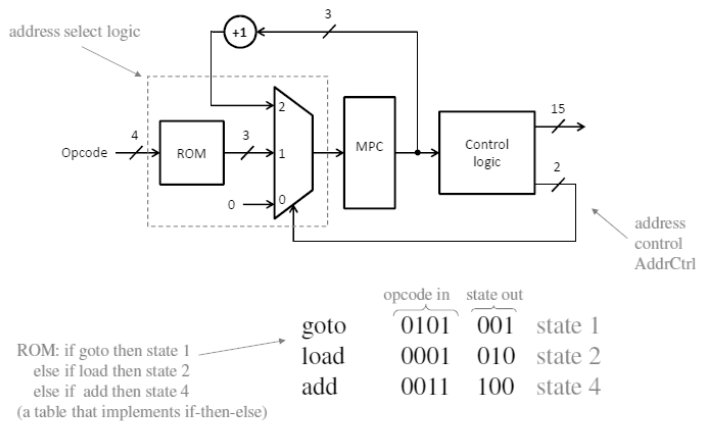
\includegraphics[scale=0.375]{img/microsequencer-implementation}
\end{figure}



\part{Intel 64 Architecture}


\section{Intel 64 Introduction}


\subsection{Memory}


\subsubsection{Registers}

\begin{table}[H]
\noindent \centering{}\texttt{\footnotesize{}}%
\begin{tabular}{cccccc}
\toprule 
\emph{\footnotesize{}Register} & \emph{\footnotesize{}64-bit} & \emph{\footnotesize{}32-bit} & \emph{\footnotesize{}16-bit} & \emph{\footnotesize{}8-bit (high)} & \emph{\footnotesize{}8-bit (low)}\tabularnewline
\midrule
{\footnotesize{}A} & \texttt{\footnotesize{}rax} & \texttt{\footnotesize{}eax} & \texttt{\footnotesize{}ax} & \texttt{\footnotesize{}ah} & \texttt{\footnotesize{}al}\tabularnewline
{\footnotesize{}B} & \texttt{\footnotesize{}rbx} & \texttt{\footnotesize{}ebx} & \texttt{\footnotesize{}bx} & \texttt{\footnotesize{}bh} & \texttt{\footnotesize{}bl}\tabularnewline
{\footnotesize{}C} & \texttt{\footnotesize{}rcx} & \texttt{\footnotesize{}ecx} & \texttt{\footnotesize{}cx} & \texttt{\footnotesize{}ch} & \texttt{\footnotesize{}cl}\tabularnewline
{\footnotesize{}D} & \texttt{\footnotesize{}rdx} & \texttt{\footnotesize{}edx} & \texttt{\footnotesize{}dx} & \texttt{\footnotesize{}dh} & \texttt{\footnotesize{}dl}\tabularnewline
{\footnotesize{}Source Index} & \texttt{\footnotesize{}rsi} & \texttt{\footnotesize{}esi} & \texttt{\footnotesize{}si} &  & \texttt{\footnotesize{}sil}\tabularnewline
{\footnotesize{}Destination Index} & \texttt{\footnotesize{}rdi} & \texttt{\footnotesize{}edi} & \texttt{\footnotesize{}di} &  & \texttt{\footnotesize{}dil}\tabularnewline
{\footnotesize{}Stack Pointer} & \texttt{\footnotesize{}rsp} & \texttt{\footnotesize{}esp} & \texttt{\footnotesize{}sp} &  & \texttt{\footnotesize{}spl}\tabularnewline
{\footnotesize{}Base Pointer} & \texttt{\footnotesize{}rbp} & \texttt{\footnotesize{}ebp} & \texttt{\footnotesize{}bp} &  & \texttt{\footnotesize{}bpl}\tabularnewline
{\footnotesize{}Instruction Pointer} & \texttt{\footnotesize{}rip} &  &  &  & \tabularnewline
{\footnotesize{}Flags} & \texttt{\footnotesize{}rflags} &  &  &  & \tabularnewline
\bottomrule
\end{tabular}
\end{table}



\paragraph{Instruction Pointer Register}
\begin{itemize}
\item Holds next instruction to be executed.
\item Rarely manipulated directly by programs.
\item Used implicitly by instructions such as \texttt{call}, \texttt{jmp}
and \texttt{ret}.
\item Used to implement if and while statements, method calls.
\end{itemize}

\paragraph{Flags Register}
\begin{itemize}
\item 6: Zero flag, 1 if result is 0.
\item 7: Sign flag: Most signifcant bit of result (sign bit for signed int).
\item 11: Overflow flag: 1 if signed result overflows.
\item 0: Carry flag: 1 if unsigned result overflows.
\item 2: Parity flag: 1 if LS byte of result contains even number of bits.
\end{itemize}

\subsubsection{Main Memory}

Byte addresable, little endian, non-aligned access is allowed.


\subsection{Instructions}

Generally have the form \texttt{label: opcode Destination, Source
; comments}.


\paragraph{Global Variables}

Examples:

\noindent 
\begin{lstlisting}[basicstyle={\footnotesize\ttfamily},frame=single]
age        dw           21      ; word with val 21
total      dd           999     ; doubleword with val 999
message    db           "hello" ; 5-byte string hello
sequence   dw           1,2,3   ; 3 words with vals 1,2,3
array      times 100 dw 33      ; 100 words with val 33

little     resw         100     ; reserve 100 words
big        resd         1000    ; reserve 1000 dwords

dozen      equ          12      ; defines constant `dozen'
\end{lstlisting}



\section{Addressing Modes}

Example assembly instructions:

\noindent 
\begin{lstlisting}[basicstyle={\footnotesize\ttfamily},frame=single]
mov   rax, [rpb+4]   ; rax = memory16[rpb + 4]
add   ax, [bx]       ; ax = ax + memory16[bx]
sub   rax, 45        ; rax = rax - 45
\end{lstlisting}



\paragraph{Register Operands}

E.g. \texttt{rax}, \texttt{eax}, \texttt{dx}, \texttt{al}, \texttt{si},
\texttt{bp}.

Operand is value of specified register. Note dest and src operands
usually need to be same size.


\paragraph{Immediate Operands}

E.g. \texttt{23}, \texttt{67H}, \texttt{101010B}, \texttt{`A'}

Operand is the constant value specified directly. Not normally applicable
for dest operands.


\paragraph{Memory Operands}

\texttt{{[}BaseReg + Scale {*} IndexReg + Disp{]}} where:
\begin{enumerate}
\item \texttt{BaseReg} can be any register
\item \texttt{Scale} $\in\left\{ 1,2,4,8\right\} $
\item \texttt{IndexReg} can be any register except \texttt{rsp}
\item \texttt{Disp} is a 64-bit constant
\end{enumerate}
Note that order is unimportant. Size of operands normally inferred.
\begin{enumerate}
\item \texttt{{[}Disp{]}}: \emph{Direct addressing}: address given by constant
value. Allows access to global variables.
\item \texttt{{[}BaseReg{]}}: \emph{Register indirect}: address given by
contents of register. Dynamically points to variables in memory based
on computed addresses.
\item \texttt{{[}BaseReg + Disp{]}}: \emph{Register Relative}: Sum gives
address. \texttt{Disp} can be negative. Can be used to access object
fields, array elements.
\item \texttt{{[}BaseReg + IndexReg{]}}: \emph{Based-Indexed}: Can be used
to access array elements, where start of array dynamically determined.
\item \texttt{{[}BaseReg + IndexReg + Disp{]}}: \emph{Based Relative Index}:
Can be used to access arrays of objects, arrays within objects, arrays
on stack.
\item \texttt{{[}Scale {*} IndexReg + Disp{]}}: \emph{Scaled-Indexed}: Efficient
access to array elements when element size is 1, 2, 4 or 8 bytes.
\item \texttt{{[}BaseReg + Scale {*} IndexReg + Disp{]}}: Efficient access
to array elements within objects / on the stack.
\end{enumerate}

\section{Programming}


\subsection{Arithmetic Instructions}

\begin{table}[H]
\noindent \centering{}\texttt{\footnotesize{}}%
\begin{tabular}{llll}
\toprule 
\multicolumn{2}{l}{\emph{Instruction}} & \emph{Operation} & \emph{Description}\tabularnewline
\midrule
\texttt{add} & \texttt{dst, src} & dst = dst + src & Add\tabularnewline
\texttt{sub} & \texttt{dst, src} & dst = dst - src & Subtract\tabularnewline
\texttt{cmp} & \texttt{dst, src} & dst - src & Compare and set \texttt{RFLAGS}\tabularnewline
\texttt{inc} & \texttt{opr} & opr = opr + 1 & Increment by 1\tabularnewline
\texttt{dec} & \texttt{opr} & opr = opr - 1 & Decrement by 1\tabularnewline
\texttt{neg} & \texttt{opr} & opr = - opr & Negate\tabularnewline
\texttt{imul} & \texttt{dst, src} & dst = dst {*} src & Integer multiply\tabularnewline
\texttt{imul} & \texttt{dst, src, imm} & dst = src {*} imm & Integer multiply\tabularnewline
\multirow{2}{*}{\texttt{idiv}} & \multirow{2}{*}{\texttt{opr}{*}} & al = ax \textbf{div} opr & \multirow{2}{*}{Integer divide}\tabularnewline
 &  & ah = ax \textbf{mod} opr & \tabularnewline
\multirow{2}{*}{\texttt{idiv}} & \multirow{2}{*}{\texttt{opr}{*}} & ax = (dx:ax) \textbf{div} opr & \multirow{2}{*}{Integer divide}\tabularnewline
 &  & dx = (dx:ax) \textbf{mod} opr & \tabularnewline
\texttt{sal} & \texttt{dst, n} & dst = dst {*} $2^{n}$ & Shift arithmetic left\tabularnewline
\texttt{sar} & \texttt{dst, n} & dst \textbf{div} dst {*} $2^{n}$ & Shit arithmetic right\tabularnewline
\texttt{cbw} &  & ax = al & Convert byte to word\tabularnewline
\texttt{cwde} &  & eax = ax & Convert word to doublewd\tabularnewline
\texttt{cdq} &  & edx:eax = eax & Conver double to quadwd\tabularnewline
\texttt{cqo} &  & rdx:rax = rax & Extend quadword\tabularnewline
\bottomrule
\end{tabular}
\end{table}


{*} Must be register or memory only. \texttt{idiv} works similarly
in 32 and 64 bits (using extended registers).


\paragraph{Overflows}
\begin{enumerate}
\item E.g. occurs on signed byte additions where $A+B>127$ or $A+B<-128$. 
\item Sets overflow flag in \texttt{RFLAGS}.
\item We can use \texttt{jo ov\_label ; Jump to ov\_label if overflow}.
\end{enumerate}

\paragraph{Division by Zero}

Check the zero flag:

\noindent 
\begin{lstlisting}[basicstyle={\footnotesize\ttfamily},frame=single]
cmp    bh, 0      ; compare divisor with 0
je     zd_label   ; jump to zd_label if divisor is zero
idiv   bh         ; otherwise go ahead with division
\end{lstlisting}



\subsection{Logical Instructions}

\begin{table}[H]
\noindent \centering{}\texttt{\footnotesize{}}%
\begin{tabular}{llll}
\toprule 
\multicolumn{2}{l}{\emph{Instruction}} & \emph{Operation} & \emph{Description}\tabularnewline
\midrule
\texttt{and} & \texttt{dst, src} & dst = dst \& src & Bitwise and\tabularnewline
\texttt{test} & \texttt{dst, src} & dst \& src & Bitwise and, set \texttt{RFLAGS}\tabularnewline
\texttt{or} & \texttt{dst, src} & dst = dst \textbar{} src & Bitwise or\tabularnewline
\texttt{xor} & \texttt{dst, src} & dst = dst \textasciicircum{} src & Bitwise xor\tabularnewline
\texttt{not} & \texttt{opr} & opr = \textasciitilde{} opr & Bitwise not\tabularnewline
\bottomrule
\end{tabular}
\end{table}

\begin{enumerate}
\item \texttt{and} clears specific (0 in \texttt{src}) bits in \texttt{dst}.
\item \texttt{or} sets specific (1 in \texttt{src}) bits in \texttt{dst}.
\item \texttt{xor} toggles specific (1 in \texttt{src}) bits in \texttt{dst}.
\end{enumerate}

\paragraph{Boolean Expressions}

Represent boolean using a full byte: 0 for false, true otherwise.


\subsection{Jump Instructions}

\begin{table}[H]
\noindent \centering{}\texttt{\footnotesize{}}%
\begin{tabular}{llll}
\toprule 
\multicolumn{2}{l}{\emph{Instruction}} & \emph{Flag Condition} & \emph{Description}\tabularnewline
\midrule
\texttt{jmp} & \texttt{label} & None & Jump\tabularnewline
\texttt{je/jz} & \texttt{label} & ZF = 1 & Jump if zero (equal)\tabularnewline
\texttt{jne/jnz} & \texttt{label} & ZF = 0 & Jump if not zero (not equal)\tabularnewline
\texttt{jg} & \texttt{label} & ZF = 0 and SF = 0 & Jump if greater than\tabularnewline
\texttt{jge} & \texttt{label} & SF = 0 & Jump if greater than or equal to\tabularnewline
\texttt{jl} & \texttt{label} & SF = 1 & Jump if less than\tabularnewline
\texttt{jle} & \texttt{label} & ZF = 1 or SF = 1 & Jump if less than or equal to\tabularnewline
\bottomrule
\end{tabular}
\end{table}



\paragraph{If-then-else}

\texttt{if (age \textless{} 100) then s1 else s2}:

\noindent 
\begin{lstlisting}[basicstyle={\footnotesize\ttfamily},frame=single]
if:    cmp word[age], 100
       jge else
       ; s1
       jmp endif
else:  ; s2
endif:
\end{lstlisting}



\paragraph{While loop}

\texttt{while (age \textless{} 100) s}:

\noindent 
\begin{lstlisting}[basicstyle={\footnotesize\ttfamily},frame=single]
while:    cmp word[age], 100
          jge endwhile
          ; s
          jmp while
endwhile:
\end{lstlisting}



\paragraph{For loop}

\texttt{for (age = 1; age \textless{} 100; age++) s}:

\noindent 
\begin{lstlisting}[basicstyle={\footnotesize\ttfamily},frame=single]
for:    mov word[age], 1
next:   cmp word[age], 100
        jge endfor
        ; s
        inc word[age]
        jmp next
endfor: 
\end{lstlisting}



\subsection{Methods}
\begin{enumerate}
\item \emph{Jump} to the beginning of some code, \emph{execute} it, \emph{return}
(possibly with results) to where called from.
\item Need to consider: \emph{parameters}, \emph{local variable}, \emph{nested
and recursive method calls}.
\end{enumerate}

\subsubsection{Stacks}
\begin{enumerate}
\item Last-in, first-out: two basic operations, \texttt{push} and \texttt{pop}.
\item \texttt{rsp} (stack pointer) points to top of stack.
\item \texttt{rbp} (base pointer) keeps track of data on the stack.
\end{enumerate}
NB: \emph{Stack grows downwards}, from higher addresses to lower addresses.

\begin{table}[H]
\noindent \centering{}\texttt{\footnotesize{}}%
\begin{tabular}{llll}
\toprule 
\multicolumn{2}{l}{\emph{Instruction}} & \emph{Operation} & \emph{Description}\tabularnewline
\midrule
\multirow{2}{*}{\texttt{push}} & \multirow{2}{*}{\texttt{word\_opr}{*}} & rsp = rsp - 2 & \multirow{2}{*}{Push word onto stack}\tabularnewline
 &  & memory{[}rsp{]} = word\_opr & \tabularnewline
\multirow{2}{*}{\texttt{pop}} & \multirow{2}{*}{\texttt{word\_opr}{*}} & word\_opr = memory{[}rsp{]} & \multirow{2}{*}{Pop word off of stack}\tabularnewline
 &  & rsp = rsp + 2 & \tabularnewline
\multirow{2}{*}{\texttt{pushfq}} & \multirow{2}{*}{} & ZF = 0 & \multirow{2}{*}{Push \texttt{RFLAGS} onto stack}\tabularnewline
 &  & ZF = 0 and SF = 0 & \tabularnewline
\multirow{2}{*}{\texttt{popfq}} & \multirow{2}{*}{} & SF = 0 & \multirow{2}{*}{Pop \texttt{RFLAGS} off stack}\tabularnewline
 &  & SF = 1 & \tabularnewline
\multirow{2}{*}{\texttt{call}} & \multirow{2}{*}{\texttt{method}} & \texttt{push rip} & Push return address and\tabularnewline
 &  & \texttt{jmp method} & jump to method code\tabularnewline
\multirow{2}{*}{\texttt{ret}} & \multirow{2}{*}{} & \multirow{2}{*}{\texttt{pop rip}} & Pop return address into\tabularnewline
 &  &  & \texttt{rip} (so jumping back)\tabularnewline
\bottomrule
\end{tabular}
\end{table}


{*} Quadwords can also be pushed and popped. No other operand sizes
are allowed.


\subsubsection{Calling Convention}

\begin{table}[H]
\noindent \centering{}{\footnotesize{}}%
\begin{tabular}{lll}
\toprule 
\multicolumn{1}{l}{} & \emph{Calling method (Caller)} & \emph{Called method (Callee)}\tabularnewline
\midrule
1. & Push parameters, last to first. & \tabularnewline
2. & Push object instance. & \tabularnewline
3. & Jump to (call) method. & \tabularnewline
4. &  & Save registers on stack.\tabularnewline
5. &  & Execute body of method.\tabularnewline
6. &  & Copy result to \texttt{eax} or \texttt{rax}.\tabularnewline
7. &  & Restore registers from stack.\tabularnewline
8. &  & Jump back (return) from method.\tabularnewline
9. & Remove object instance from stack. & \multirow{1}{*}{}\tabularnewline
10. & Remove parameners from stack. & \tabularnewline
11. & Use method result. & \tabularnewline
\bottomrule
\end{tabular}
\end{table}



\paragraph{Local Variables}

\textbf{Callee} makes space for local variables:

\noindent 
\begin{lstlisting}[basicstyle={\footnotesize\ttfamily},frame=single]
push   rbp           ; push caller's frame pointer onto stack
mov    rbp, rsp      ; set frame pointer to current stack pointer
sub    rsp, nbytes   ; allocate nbytes for local vars
\end{lstlisting}


and then de-allocates these variables:

\noindent 
\begin{lstlisting}[basicstyle={\footnotesize\ttfamily},frame=single]
mov    rsp, rbp      ; restore stack pointer
pop    rbp           ; restore caller's frame pointer
\end{lstlisting}



\paragraph{Array and object parameters}

We push the start \emph{address} rather than its value. We can use
\texttt{lea} (load effective address) to do this: \texttt{lea dstreg,
{[}BaseReg + Scale {*} IndexReg + Disp{]}}.


\paragraph{Object Method Calls}

Need to be translated as if they were written without a class.

\begin{table}[H]
\textbf{Example: Caller}

\noindent \begin{minipage}[t]{0.2\textwidth}
\begin{lstlisting}[basicstyle={\scriptsize\ttfamily},breaklines=true,keywords={loop, exit, when, end}]
coord point
...
point.setpos(3, 5)

/* translated to: */
coord_setpos(point, 3, 5)
\end{lstlisting}


\noindent \end{minipage}
\begin{minipage}[t]{0.3\textwidth}

\noindent \begin{centering}
\begin{lstlisting}[basicstyle={\scriptsize\ttfamily},breaklines=true,keywords={loop, exit, when, end}]
point resd 2        ; allocate point
...
push qword 5        ; push 5
push qword 3        ; push 3
push qword point    ; push @point
call coord_setpos   ; call callee
add  rsp, 24        ; restore stack pointer
\end{lstlisting}

\par\end{centering}

\noindent \centering{}\end{minipage}
\end{table}
\begin{table}[H]
\textbf{Example: Callee}

\noindent \begin{centering}
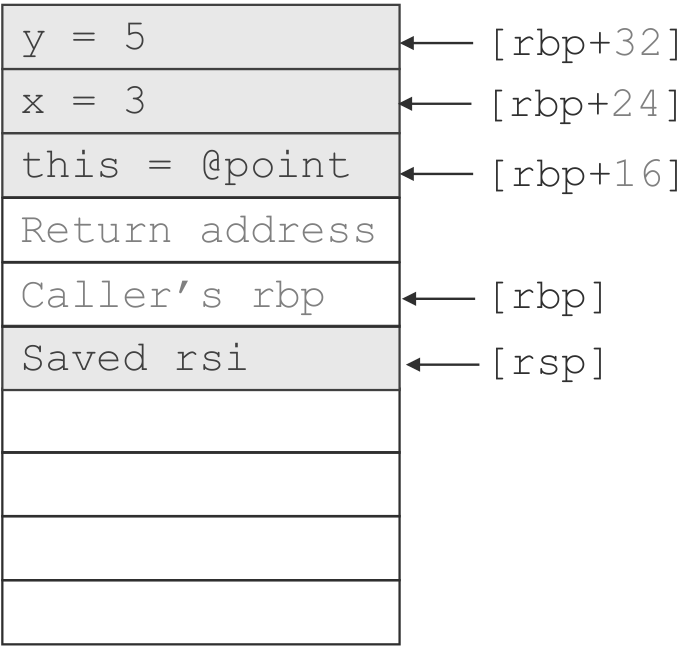
\includegraphics[scale=0.15]{img/stack}
\par\end{centering}

\noindent \begin{minipage}[t]{0.2\textwidth}
\begin{lstlisting}[basicstyle={\scriptsize\ttfamily},breaklines=true,keywords={loop, exit, when, end}]
class coord {
  int row;
  int col;
  void setpos (int x, int y) {
    row = x;
    col = y;
  }
}

/* translated to: */
void coord_setpos (coord this, int x, int y) {
  this.row = x;
  this.col = y;
}
\end{lstlisting}


\noindent \end{minipage}
\begin{minipage}[t]{0.3\textwidth}

\noindent \begin{centering}
\begin{lstlisting}[basicstyle={\scriptsize\ttfamily},breaklines=true,keywords={loop, exit, when, end}]
coord_setpos:
  push rbp             ; save frame pointer
  mov  rbp, rsp        ; setup frame pointer
  push rsi             ; save rsi
  mov  rsi, [rbp+16]   ; rsi = this
  
  mov  rax, [rbp+24]   ; rax = x
  mov  [rsi], rax      ; this.row = x
  mov  rax, [rbp+32]   ; rax = y
  mov  [rsi+4], rax    ; this.col = y

  pop  rsi             ; restore rsi
  pop  rbp             ; restore frame pointer
  ret                  ; return
\end{lstlisting}

\par\end{centering}

\noindent \centering{}\end{minipage}
\end{table}



\section{Floating Point Numbers}

Represent numbers in format $M\times2^{E}$.
\begin{itemize}
\item $M$ is the \emph{coefficient}, \emph{significand}, \emph{fraction}
or \emph{mantissa}. No. of bits determinse \emph{precision}.
\item $E$ is the \emph{exponent} or \emph{characteristic}. No. of bits
determines \emph{range}.
\item $2$is the \emph{radix} or \emph{base}.
\end{itemize}

\paragraph{Zones of Expressibility}

E.g. with signed 3-digit coefficient and signed 2-digit exponent:

\begin{figure}[H]
\noindent \centering{}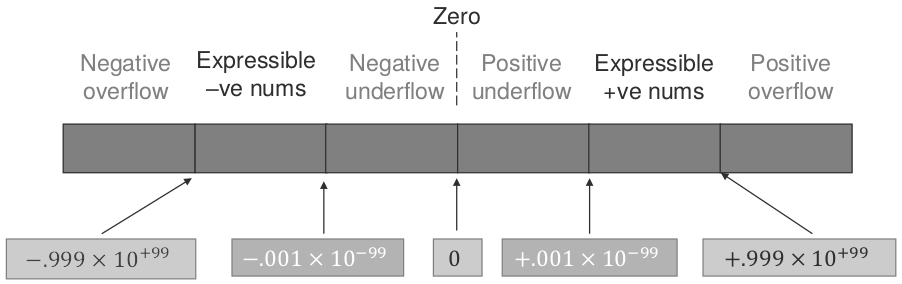
\includegraphics[scale=0.3]{img/floatrange}
\end{figure}



\paragraph{Floating Point vs Real Numbers}
\begin{enumerate}
\item Floating points have a finite range ad a finite number of values.
\item The gap between numbers varies.
\item Incorrect results are possible.
\end{enumerate}

\paragraph{Normalised Form}

We normalise coefficients in the range $\left[1,\dots R\right)$ where
$R$ is the base.


\paragraph{Binary Fractions}

E.g. decimal value of \textbf{0.01101}?

\begin{table}[H]
\noindent \centering{}%
\begin{tabular}{cccccc}
\toprule 
32 & 16 & 8 & 4 & 2 & 1\tabularnewline
\textbf{.} & \textbf{0} & \textbf{1} & \textbf{1} & \textbf{0} & \textbf{1}\tabularnewline
\bottomrule
\end{tabular}$=\frac{8+4+1}{32}=\frac{13}{32}$
\end{table}


E.g. binary value of \textbf{0.6875}?
\[
=\frac{1.375}{2}=\frac{1}{2}+\frac{0.75}{4}=\frac{1}{2}+\frac{1.5}{8}=\frac{1}{2}+\frac{1}{8}+\frac{1}{16}=0.1011
\]



\paragraph{Multiplication}

Multiply coefficents, add exponents, normalise result.


\paragraph{Addition}

Need to align \emph{smaller exponent}, by shifting its coefficient
the corresponding number of digits to the right.


\paragraph{Comparing}

Due to potential for inexact results, $a=b$ should be adjusted to
$b-\epsilon<a<b+\epsilon$. Or calculated closeness based on relative
sizes.


\paragraph{Truncation and Rounding}

If result is too large to store in coefficent truncate (biased error)
or round (unbiased).


\paragraph{Exponent Overflow and Underflow}

Set value as infinity / zero or raise an exception.


\subsection{IEEE Floating Point Standard}

\noindent \begin{center}
\begin{tabular}{ccc}
\toprule 
Sign $S$ & Exponent $E$ & Significand $F$\tabularnewline
1 bit & 8 (\emph{11}) bits & 23 (\emph{52}) bits\tabularnewline
\bottomrule
\end{tabular}
\par\end{center}


\paragraph{Single Precision}
\begin{enumerate}
\item Represented value is $\pm1.F\times2^{E-127}$.
\item First significand bit (1) is hidden.
\item Note that exponents stored in excess-127 values.
\end{enumerate}

\paragraph{Double Precision}

Value is $\pm1.F\times2^{E-1023}$.


\paragraph{Conversion to IEEE Format}

E.g. 42.6875 in single precision format.
\begin{enumerate}
\item Convert to binary number: 10 1010.1011
\item Normalise : 1.0101 0101 1$\times2^{5}$
\item Significand field: 0101 0101 1000 0000 0000 000
\item Exponent field: 5 + 127 = 132 = 1000 0100
\end{enumerate}
Gives %
\begin{tabular}{ccc}
\toprule 
$S$ & $E$ & $F$\tabularnewline
0 & 1000 0100 & 0101 0101 1000 0000 0000 000\tabularnewline
\bottomrule
\end{tabular} or 422A C000.


\paragraph{Conversion from IEEE Format}

E.g. BEC0 0000 or 1 01111101 10000000000000000000000 from single precision
format.
\begin{enumerate}
\item Exponent field: 125 - 127 = - 2
\item Significand field: 1.1
\item Add sign bit: - 1.1$\times2^{-2}$ = - 0.25 - 0.125 = - 0.375
\end{enumerate}

\paragraph{Addition}
\begin{enumerate}
\item Shift smaller number to the right so that exponents are the same.
\item Sum significands.
\end{enumerate}

\paragraph{Special Values}
\begin{enumerate}
\item \textbf{Zero} has 0 exponent and 0 significand.
\item \textbf{Denormalised numbers} ($0.F\times2^{-126}$) have 0 exponent.
\item \textbf{Infinity} has 255 exponent and 0 significand.
\item \textbf{NaN} has 255 exponent.
\item \textbf{Normalised numbers} have 1..254 exponent.
\end{enumerate}
Infinity and NaN do what you expect under mathematical operations.


\section{Input and Output}


\paragraph{I/O Controllers}
\begin{enumerate}
\item Provide CPU with a programming interface.
\item \emph{Data ports} used for passing data to / from CPU.
\item \emph{Control ports} used to issue I/O commands and check device status.
\end{enumerate}

\paragraph{I/O Addressing I : Seperate Address Space}
\begin{enumerate}
\item I/O ports have their own small address space. Architecture provides
commands to access it.
\item Control bus signals if transfer is for I/O or main memory address
space.
\item Intel 64 provides 64K 8-bit I/O ports.
\end{enumerate}
\noindent 
\begin{lstlisting}[basicstyle={\footnotesize\ttfamily},frame=single]
in    ax, 20   ; copy 16 bits from I/O port 20 to ax 
out   35, al   ; copy 8 bits from al to I/O port 35
\end{lstlisting}



\paragraph{I/O Addressing I : Memory Mapped I/O}
\begin{enumerate}
\item I/O ports appear as normal memory locations.
\item Any instruction acting on memory operands can be used on I/O ports.
\item Intel 64 also supports this.
\end{enumerate}

\paragraph{Four I/O Schemes}
\begin{enumerate}
\item \emph{Programmed I/O}: Continually polls a control port until it's
ready, then transfers.

\begin{enumerate}
\item Pros: Simple to program and guarantees response times.
\item Cons: Poor CPU utilisation, awkward to handle multiple devices.
\end{enumerate}
\item \emph{Interrupt-driven I/O}: Initiate transfer and then do something
else, interrupt CPU when transfer is complete. Control then transferred
to interrupt handler.

\begin{enumerate}
\item Cons: Need to save and restore CPU state. Bad for high-speed high-data
volume devices that might lose data if they are not serviced quickly
enough. Bad if devices continually require attention.
\end{enumerate}
\item \emph{DMA I/O}: Initiate large data block transfer. CPU writes start
address of block, number of bytes, and direction of transfer to DMA's
I/O ports and issues start command. DMA controller transfers block
of data to main memory without direct CPU intervention. Interrupts
CPU when completed.

\begin{enumerate}
\item Pro: Greatly reduces interrupts.
\end{enumerate}
\item \emph{I/O processor}: Delegate I/O tasks to dedicated processor. Much
more powerful solution.
\end{enumerate}

\paragraph{Operating Systems: Concurrency}

Interleaves processes. Operating system is a scheduler that puts processes
(threads) in different states (using interrupts).


\subsection{Interrupts}


\paragraph{Locating Interrupt Handler}
\begin{enumerate}
\item Device that wishes to interrupt CPU sends an interrupt signal to the
CPU along with a \emph{interrupt vector number}.
\item Interrupt vector number indexes \emph{interrupt descriptor table}.
\item Start address of IDT is held in special CPU register called \emph{IDT
base register}.
\end{enumerate}

\paragraph{Calling the Interrupt Handler}

The Intel 64 CPU:
\begin{enumerate}
\item Completes the executing instruction.
\item Pushes RFLAGS onto the stack.
\item Clears the interrupt flag bit in the RFLAGS register.
\item Push the CS register and return address
\item Jump to interrupt handler using IDT.
\end{enumerate}
Handler executes \texttt{iret} which restores state of RFLAGS, CS
and RIP and jumps to return address on stack. \emph{Preserving registers
is duty of handler}.


\paragraph{Enabling and Disabling Interrupts}
\begin{enumerate}
\item Interrupts automatically disabled on entering handler.
\item Interrupts can be re-enabled by setting IF (interrupt enable flag)
with \texttt{sti}.
\item Interrupts can be disabled using \texttt{cli}.
\end{enumerate}

\paragraph{Drivers}
\begin{enumerate}
\item Devices controlled by readiny writing to I/O ports (memory locations
in memory-mapped I/O).
\item Completion of I/O request signalled by sending interrupt vector number
whiich causes CPU to call device's interrupt handler.
\item \emph{Top half} (\emph{interrupt handler}) services interrupt - check
for errors and copies data to / from memory and shares it with bottom
half.
\item \emph{Bottom half} runs as a \emph{schedulable thread} within the
OS and interracts with the device via I/O ports, the top half (via
shared memory) and the user-level process.
\end{enumerate}

\paragraph{Types of Interrupt}
\begin{enumerate}
\item External I/O Device-generated (vectors \emph{32-255}): I/O devices
sends interrupt via buses. The only asynchronous type.
\item CPU-generated (\emph{0-18}) : Attempt to execute illegal operation.
\item Software-generated: Generated by instruction.
\end{enumerate}

\paragraph{Software Interrupts (System Calls / Traps)}
\begin{enumerate}
\item \texttt{syscall} used to call operating system functions.
\item System call number held in \texttt{rax}. E.g. 0 = read from standard
input, 1 = write to standard output.
\item Parameters held in \texttt{rdi}, \texttt{rsi}, \texttt{rdx}, \texttt{rcx},
\texttt{r8}, \texttt{r9}.
\item Result passed into \texttt{rax}.\end{enumerate}

\end{document}
